\begin{sfragment}{Introduction}
  The \pkg{notesslides} document class is derived from |beamer.cls|~\cite{beamerclass:on},
it adds a ``notes version'' for course notes that is more suited to printing than the one
supplied by |beamer.cls|.

The \pkg{notesslides} class takes the notion of a slide frame from Till Tantau's excellent
\pkg{beamer} class and adapts its notion of frames for use in the \sTeX and \omdoc. To
support semantic course notes, it extends the notion of mixing frames and explanatory
text, but rather than treating the frames as images (or integrating their contents into
the flowing text), the \pkg{notesslides} package displays the slides as such in the course
notes to give students a visual anchor into the slide presentation in the course (and to
distinguish the different writing styles in slides and course notes).

In practice we want to generate two documents from the same source: the slides for
presentation in the lecture and the course notes as a narrative document for home
study. To achieve this, the \pkg{notesslides} class has two modes: \emph{slides mode} and
\emph{notes mode} which are determined by the package option. 
\end{sfragment}

\begin{sfragment}{Package Options}
  The \pkg{notesslides} class takes a variety of class options:
  \begin{itemize}
  \item
    \begin{variable}{slides,notes} The options |slides| and |notes| switch between
      slides mode and notes mode (see \sref{sec:user:notesslides}).
    \end{variable}
  \item
    \begin{variable}{sectocframes} If the option |sectocframes| is given, then for the
      |sfragment|s, special frames with the |sfragment| title (and number) are generated.
    \end{variable}
  \item
    \begin{variable}{frameimages,fiboxed}
      If the option |frameimages| is set, then slide mode also shows the
      |\frameimage|-generated frames (see \sref{sec:user:frameimage}). If also the
      |fiboxed| option is given, the slides are surrounded by a box.
    \end{variable}
  \end{itemize}
\end{sfragment}

\begin{sfragment}[id=sec:user:notesslides]{Notes and Slides}

\begin{environment}{frame}
  Slides are represented with the |frame| environment just like in the \pkg{beamer} class,
  see~\cite{Tantau:ugbc} for details.
\end{environment}

\begin{environment}{note}
  The \pkg{notesslides} class adds the |note| environment for encapsulating the course
  note fragments.\footnote{MK: it would be very nice, if we did not need this environment,
    and this should be possible in principle, but not without intensive LaTeX
    trickery. Hints to the author are welcome.}
\end{environment}
  
\begin{dangerbox}
  Note that it is essential to start and end the |notes| environment at the start of the
  line -- in particular, there may not be leading blanks -- else {\LaTeX} becomes confused
  and throws error messages that are difficult to decipher.
\end{dangerbox}

By interleaving the |frame| and |note| environments, we can build course notes as shown
here:

\begin{latexcode}
\ifnotes\maketitle\else
\frame[noframenumbering]\maketitle\fi

\begin{note}
  We start this course with ...
\end{note}

\begin{frame}
  \frametitle{The first slide}
  ...
\end{frame}
\begin{note}
  ... and more explanatory text
\end{note}

\begin{frame}
  \frametitle{The second slide}
  ...
\end{frame}
...
\end{latexcode}

\begin{function}{\ifnotes}
  Note the use of the |\ifnotes| conditional, which allows different treatment between
  |notes| and |slides| mode -- manually setting |\notestrue| or |\notesfalse| is strongly
  discouraged however.
\end{function}
 
\begin{dangerbox}
  We need to give the title frame the |noframenumbering| option so that the frame
  numbering is kept in sync between the slides and the course notes.
\end{dangerbox}

\begin{dangerbox}
  The \pkg{beamer} class recommends not to use the |allowframebreaks| option on frames
  (even though it is very convenient). This holds even more in the |notesslides| case: At
  least in conjunction with |\newpage|, frame numbering behaves funnily (we have tried to
  fix this, but who knows).
\end{dangerbox}
\end{sfragment}

\begin{function}{\inputref*}
  If we want to transclude a the contents of a file as a note, we can use a new variant
  |\inputref*| of the |\inputref| macro: |\inputref*{foo}| is equivalent to
  |\begin{note}\inputref{foo}\end{note}|.
\end{function}

\begin{environment}{nparagraph, nparagraph, ndefinition, nexample, nsproof, nassertion}
  There are some environments that tend to occur at the top-level of |note|
  environments. We make convenience versions of these: e.g. the |nparagraph| environment
  is just an |sparagraph| inside a |note| environment (but looks nicer in the source,
  since it avoids one level of source indenting). Similarly, we have the |nfragment|,
  |ndefinition|, |nexample|, |nsproof|, and |nassertion| environments.
\end{environment}

\begin{sfragment}{Customizing Header and Footer Lines}
  The \pkg{notesslides} package and class comes with a simple default theme named
  \pkg{sTeX} that provided by the \pkg{beamterthemesTeX}. It is assumed as the default
  theme for \sTeX-based notes and slides.
  The result in |notes| mode (which is like the |slides| version except that the slide
  hight is variable) is
  
  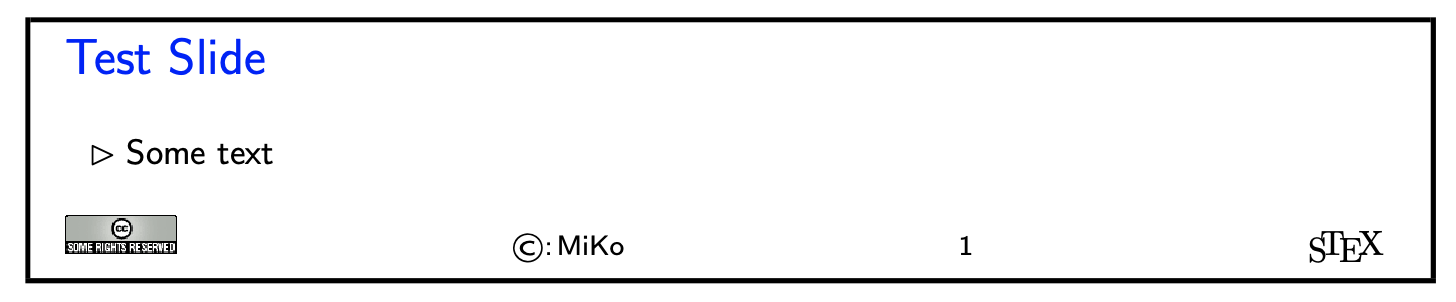
\includegraphics[width=.95\textwidth]{\libfolder{img/notes-frame}}
  
The footer line can be customized. In particular the logos. 

\begin{function} {\setslidelogo}
  The default logo provided by the \pkg{notesslides} package is the {\sTeX} logo it can be
  customized using |\setslidelogo{|\meta{logo name}|}|.
\end{function}

\begin{function}{\setsource}
  The default footer line of the \pkg{notesslides} package mentions copyright and
  licensing. In \pkg{notesslides} |\source| stores the author's name as the copyright
  holder. By default it is the author's name as defined in the |\author| macro in the
  preamble.  |\setsource{|\meta{name}|}| can change the writer's name.
\end{function}

\begin{function}{\setlicensing}
  For licensing, we use the Creative Commons Attribuition-ShareAlike license by default to
  strengthen the public domain. If package |hyperref| is loaded, then we can attach a
  hyperlink to the license logo. |\setlicensing[|\meta{url}|]{|\meta{logo name}|}| is used
  for customization, where \meta{url} is optional.
\end{function}
\end{sfragment}

\begin{sfragment}[id=sec:user:frameimages]{Frame Images}
 Sometimes, we want to integrate slides as images after all -- e.g. because we already
have a PowerPoint presentation, to which we want to add \sTeX notes.

\begin{function}{\frameimage,\mhframeimage}
  In this case we can use |\frameimage[|\meta{opt}|]{|\meta{path}|}|, where \meta{opt} are
  the options of |\includegraphics| from the \pkg{graphicx} package~\cite{CarRah:tpp99}
  and \meta{path} is the file path (extension can be left off like in
  |\includegraphics|). We have added the |label| key that allows to give a frame label
  that can be referenced like a regular |beamer| frame.

The |\mhframeimage| macro is a variant of |\frameimage| with repository support. Instead
of writing
\begin{latexcode}
\frameimage{\MathHub{fooMH/bar/source/baz/foobar}}
\end{latexcode}
  we can simply write (assuming that |\MathHub| is defined as above)
\begin{latexcode}
\mhframeimage[fooMH/bar]{baz/foobar}
\end{latexcode}
  Note that the |\mhframeimage| form is more semantic, which allows more advanced document
management features in \textsf{MathHub}.
\end{function}

If |baz/foobar| is the ``current module'', i.e. if we are on the \textsf{MathHub} path
\ldots|MathHub/fooMH/bar|\ldots, then stating the repository in the first optional
argument is redundant, so we can just use
\begin{latexcode}
\mhframeimage{baz/foobar}
\end{latexcode}
\end{sfragment}

\begin{function}{\textwarning}
  The |\textwarning| macro generates a warning sign: \textwarning
\end{function}

In course notes, we sometimes want to point to an ``excursion'' -- material that is either
presupposed or tangential to the course at the moment -- e.g. in an appendix. The typical
setup is the following:

\begin{latexcode}
\excursion{founif}{../ex/founif}{We will cover first-order unification in}
...
\begin{appendix}\printexcursions\end{appendix}
\end{latexcode}

\begin{sfragment}[id=sec:user:excursions]{Excursions}

\begin{function}{\excursion}
  The |\excursion{|\meta{ref}|}{|\meta{path}|}{|\meta{text}|}| is syntactic sugar for

\begin{latexcode}
\begin{nparagraph}[title=Excursion]
  \activateexcursion{founif}{../ex/founif}
  We will cover first-order unification in \sref{founif}.
\end{nparagraph}
\end{latexcode}
\end{function}

\begin{function}{\activateexcursion,\printexcursion,\excursionref}
  Here |\activateexcursion{|\meta{path}|}| augments the |\printexcursions| macro by a call
  |\inputref{|\meta{path}|}|. In this way, the |\printexcursions| macro (usually in the
  appendix) will collect up all excursions that are specified in the main text.

  Sometimes, we want to reference -- in an excursion -- part of another. We can use
  |\excursionref{|\meta{label}|}| for that.
\end{function}

\begin{function}{\excursiongroup}
  Finally, we usually want to put the excursions into an |sfragment| environment and add
  an introduction, therefore we provide the a variant of the |\printexcursions| macro:
  |\excursiongroup[id=|\meta{id}|,intro=|\meta{path}|]| is equivalent to
\begin{latexcode}
\begin{note}
\begin{sfragment}[id=<id>]{Excursions}
  \inputref{<path>}
  \printexcursions
\end{sfragment}
\end{note}
\end{latexcode}
\end{function}
\end{sfragment}

\begin{dangerbox}
  When option |book| which uses |\pagestyle{headings}| is given and semantic macros are
  given in the |sfragment| titles, then they sometimes are not defined by the time the
  heading is formatted. Need to look into how the headings are made. This is a problem of
  the underlying \pkg{document-structure} package.
\end{dangerbox}

%%% Local Variables:
%%% mode: latex
%%% TeX-master: "../stex-manual"
%%% End:
